\documentclass[11pt,a4paper]{report}
\usepackage[utf8]{inputenc}
\usepackage[croatian]{babel}
\usepackage{amsmath, amsfonts, amssymb}
\usepackage{graphicx}
\usepackage{fancyhdr}
\usepackage{color}
\usepackage {tikz}
\usepackage{pgfplots}
\usetikzlibrary {positioning}
\usepackage{tocloft}
\usepackage[hidelinks]{hyperref}
\usepackage[section]{placeins}
\usepackage[final]{pdfpages}
\bibliographystyle{ieeetr}%ieeetr, abbrv
\renewcommand{\cftsecleader}{\cftdotfill{\cftdotsep}}

\usepackage[blocks]{authblk}% The option is for block layout

\newcommand{\kolegij}{}
\newcommand{\naslovRada}{Proračun i konstrukcija 1-stupnjskog reduktora s cilindričnim ravnim zubima \\ {\large Timski projektni zadatak}} 
\newcommand{\mailFriendlynaslovRada}{Konstrukcije - projektni zadatak}

%\author{
%Kristijan Cetina \\{\small JMBAG: 2424011721} \\ {\href{mailto:kcetina@politehnika-pula.hr?subject=\mailFriendlynaslovRada}{{\footnotesize kcetina@politehnika-pula.hr}}} \and 
%Stjepan Grgin \\{\small JMBAG: 0112005802} \\ {\href{mailto:sgrgin@politehnika-pula.hr?subject=\mailFriendlynaslovRada}{{\footnotesize sgrgin@politehnika-pula.hr}}} \and 
%Igor Mrkić \\{\small JMBAG: 0114017089} \\ {\href{mailto:imrkic@politehnika-pula.hr?subject=\mailFriendlynaslovRada}{{\footnotesize imrkic@politehnika-pula.hr}}}
%}


\author[1]{Kristijan Cetina}
\author[2]{Stjepan Grgin}
\author[3]{Igor Mrkić}

\affil[1]{\href{mailto:kcetina@politehnika-pula.hr?subject=\mailFriendlynaslovRada}{kcetina@politehnika-pula.hr} JMBAG: 2424011721}
\affil[2]{\href{mailto:sgrgin@politehnika-pula.hr?subject=\mailFriendlynaslovRada}{sgrgin@politehnika-pula.hr} JMBAG: 0112005802}
\affil[3]{\href{mailto:imrkic@politehnika-pula.hr?subject=\mailFriendlynaslovRada}{imrkic@politehnika-pula.hr} JMBAG: 0114017089}



%\title{\kolegij \\ \naslovRada}
\title{\naslovRada}
\date{Pula, \today}

\begin{document}
\pgfplotsset{width=\textwidth,compat=newest}

\begin{titlepage}
\clearpage
\begin{center}
\begin{Huge}
POLITEHNIKA PULA\\
\end{Huge}
\begin{LARGE}
Visoka tehničko-poslovna škola s p.j.\\
Stručni studij politehnike\\
\end{LARGE}
\end{center}
\vspace{3cm}
{\let\newpage\relax\maketitle}
\thispagestyle{empty}
\vfill
\begin{abstract}
U ovom radu predstavljamo proračun strojnog sklopa - 1-stupanjskog reduktora zajedno s pripradajućim vratilima i ležajevima koji je zadan kao sastavni dio kolegija Konstrukcije.
\end{abstract}
\end{titlepage}
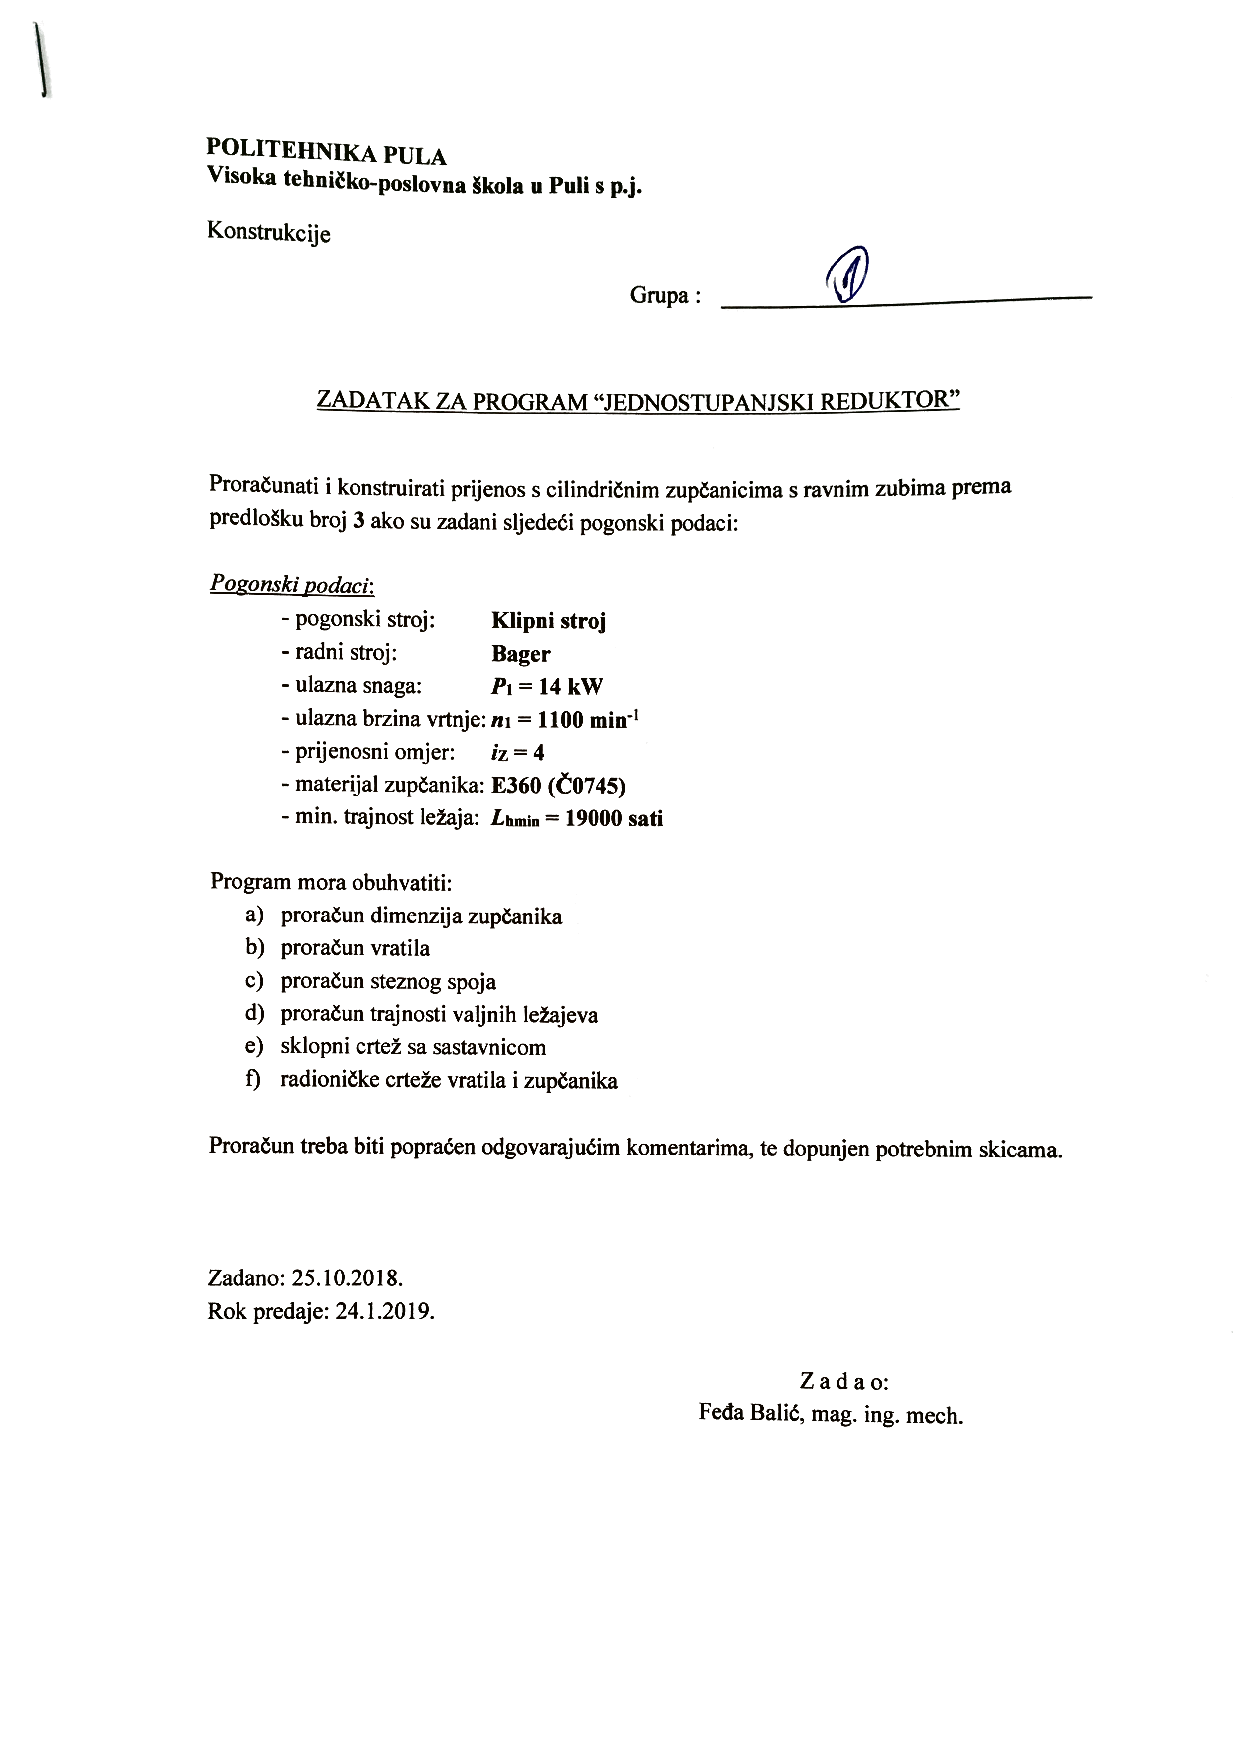
\includepdf[fitpaper]{TimskiProjektniZadatak.pdf}
\tableofcontents
\listoftables	%ako ih ima puno prebaci na kraj dokumenta
\listoffigures	%ako ih ima puno prebaci na kraj dokumenta

%Ovdje kreće rad ili može se koristiti
%\input{filename} (da nastavi pisati kako da je copy/paste) ili
%\include{filename} (da ubaci na novu stranicu. Ok za nova poglavlja i sl)
\chapter{Opis zadatka i ograničenja}
\section{Uvod}
Ovaj projektni zadatak nasto je kao obavezni zadatak u sklopu kolegija Konstrukcije koji se održava pod vodstvom Milenka Jokića, dipl.ing., predavača na stručnom studiju politehnike pri Politehnici Pula te asistenciju Feđe Balića, mag. ing. mech.

Prema zadanom predlošku (predložak 3) i zadanim podacima konstriran je 1-stupanjski reduktor s cilindričnim ravnim zubima.
Uvedena su sljedeća pojednostavljena i zanemareni sljedeći dijelovi proračuna:
\begin{itemize}
\item kontrolni pročun
\item izbor ulja za podmazivanje
\item toplinski proračun
\item određivanje stupnja korisnosti
\end{itemize}
Kod proračuna dimenzija zupčanika zanemareni su sljedeći proračuni:
\begin{itemize}
\item nosivost boka zuba
\item sigurnost na \textit{pitting} (površinski zamor)
\item nosivost korjena zuba
\end{itemize}
Kod proračuna vratila izražena je samo kontrola na plastičnu deformaciju te je zanemarena kontrola na zamor materijala.

\chapter{Proračun sklopa}
\section{Proračun dimenzija zupčanika}
Na temelju poznatih pogonskih podatak određen je minimalni diobeni promjer pogonskog zupčanika po izrazu
\begin{equation}
d_1\geq 4045 \cdot \sqrt[3]{\frac{P_1}{\psi_b \cdot n_1} \cdot \frac{i_z +i}{i_z}\cdot K_A \cdot 
K_V \cdot K_{H\alpha} \cdot K_{H\beta} \cdot \left(\frac{S_{Hmin}}{\sigma_{Hlim}}\right)^2 }\label{equ:d1minimalno}
\end{equation}
Pri čemu je $\psi_b=1$ - omjer širine zupčanika i diobenog promjera,
$P_1 \, [kW]$ - snaga pogonskog stroja,
$n_1 \, [s^{-1}]$ - broj okretaja pogonskog stroja,
$i_z$ - željeni prijenosni omjer,
$K_A=2$ - faktor primjene očitan iz tablice \cite{potrebniMaterijali},
$K_V=1$ - faktor dodatnih dinamičkih opterećenja,
$K_{H\alpha}=1$ - faktor raspodjele opterećenja na zube koji su istovremeno u zahvatu,
$K_{H\beta}=1$ - faktor raspodjele opterećenja uzduž boka zuba,
$S_{Hmin}=1,3$ - stupanj sigurnosti na površinski zamor (\textit{pitting}),
$\sigma_{H\lim}=1$ - trajna dinamička čvrstoča boka zuba na kontaktna naprezanja.

Uvrštavanje poznatih podataka u \eqref{equ:d1minimalno} dobije se minimalni diobeni promjer pogonskog zupčanika $$d_1\geq 100,3mm$$

Broj zuba pogonskog zupčanika određen je u odnosu na njegovu kutnu brzinu po izrazu
\begin{equation}
\nu=\frac{d_1 \cdot n_1 \cdot \pi}{60}\label{equ:kutnaBrzina}
\end{equation}
Uvrštavanje poznatih podataka u \eqref{equ:kutnaBrzina} dobivena je kutna brzina
$$\nu=5,77 ms^{-1}$$
te je iz tablice \cite{potrebniMaterijali} očitan mogući raspon broja zuba te je usvojen 
$$\mathbf{z_1=21}$$
Broj zuba gonjenog zupčanika je određen
\begin{align*}
z_2&=z_1 \cdot i_z\\
z_2&=21 \cdot 4\\
z_2&=\mathbf{84}
\end{align*}
Stvarni i željeni omjer su isti $$i_z=\mathbf{i_{stv}=\frac{z_2}{z_1}=4}$$
Normalni modul zuba $m_n$ je izračunat:
\begin{align*}
m_n&=\frac{d_1}{z_1}\\
m_n&=\frac{100,3}{21}\\
m_n&=4,776 mm \Rightarrow \mathbf{m_n=5 mm}
\end{align*}
Razman između osi zupčanika $a$ je određen:
\begin{align*}
a&=\frac{m_n}{2} \cdot (z_1 + z_2)\\
a&=\frac{5}{2} \cdot 105\\
a&=\mathbf{262,5mm}
\end{align*}



\newpage
\nocite{*}
\addcontentsline{toc}{chapter}{Literatura}
\bibliography{literatura}
\end{document}